In this section, we use the estimated parameters from the previous section
to analyze model in \Cref{model1} and the effect of the vaccine. Some
plausible scenarios are presented, depending on the effectiveness of the
vaccine,  as well as the rate of vaccination.

In the first instance, it has been shown that the interest region of the
state variables of the system is positively invariant and the proof can be
found in \Cref{apx:positivity_invariace}.

Now, an important concept in the analysis of the spread of diseases is the
basic reproductive number, defined as the number of secondary infections
produced by a typical infected individual, throughout his infectious period,
when in contact with a totally susceptible population. Following ideas of
\cite{Van2002}, the basic reproduction number for system in \Cref{model1} is (see
\Cref{apx:positivity_invariace})
\begin{equation}\label{Rv}
    \begin{aligned}
        R_{V} &=
            R_S + R_A
        \\
        R_S &=
            \frac{
                p \beta_S \delta_E
                (\mu + \delta_V + (1 - \epsilon)
                \lambda_V)
            }{
                (\mu + \delta_E)
                (\mu + \delta_V + \lambda_V)
                (\mu + \alpha_S)
            }
            \\
        R_A &=
            \frac{
                (1-p) \beta_A \delta_E
                (\mu + \delta_V + (1-\epsilon) \lambda_V)
            }{
                (\mu + \delta_E)
                (\mu + \delta_V + \lambda_V)
                (\mu + \alpha_A )
            }.
    \end{aligned}
\end{equation}

Note that each sum of $ R_ {V} $ represents the contribution of the symptomatic and
asymptomatic infected, respectively, to the spread of the disease.
Following the ideas of Alexander et. al. \cite{Alexander2004},
expression for $R_V$ can be rewritten as%
\begin{equation}\label{Rv2}
    R_{V} = R_0 \left(1- \frac{\epsilon \lambda_V}{(\mu+\delta_V+\lambda_V)}\right)
\end{equation}
where
\begin{equation}\label{R0}
    R_0 = \frac{p\delta_E\beta_S}{(\mu+\delta_E)(\mu+\alpha_S)} +
    \frac{(1-p) \delta_E \beta_A}{(\mu+\delta_E)(\mu + \alpha_A)}
\end{equation}
is the basic reproduction number of the system without vaccine.
Note that
$\left(1- \frac{\epsilon \lambda_V}{(\mu+\delta_V+\lambda_V)}\right)<1$. Therefore, this
factor, which enclose the  parameters corresponding to the application of the vaccine, will
allow us to modulate the value of $ R_0 $. In the  first instance, if $ R_0 <1 $,
then $ R_V <1 $. But, if $ R_0> 1 $, we ask if the application of the vaccine can
lower $R_V$ value below 1. In this sense, it is easy to prove that, if
\begin{equation}\label{condition1}
    \lambda_V>\frac{(R_0-1)(\mu+\delta_V)}{(\epsilon-1)R_0+1},
\end{equation}
%
for $\epsilon>1-(1/R_0)$, it is possible to reduce the value of $ R_V $ below one.
That is, there is a region in the parameter space in which it is possible to reduce
the value of $ R_V $ below one, considering adequate efficacy, vaccination rate and
duration of the effect of the vaccine. However, if the Inequality
\eqref{condition1} is not satisfied, it will not be possible to reduce the value of
$ R_V $ below 1.

To illustrate the aforementioned, \Cref{R0-2D} shows the regions where it is possible to
reduce the value of $ R_V $. In this case, we set all the system parameters as given in
\Cref{tbl:fixed_parameters} and with $ \delta_V = 1/180 $, leaving $ \epsilon $ and $
\lambda_V $ free.
\begin{table}[h!]
    \begin{center}
        \begin{tabular}{rl}
            \toprule
            Parameter & Value
            \\
            \midrule
            $\beta_S$ & $ \num{0.363282}$
            \\
            $\beta_A$ & $\num{0.251521}$
            \\
            $\alpha_{S}$  & $\num{0.0925069}$
            \\
            $\alpha_{A}$ & $\num{0.167504}$
            \\
            $\delta_{E}$ & $\num{0.196078}$
            \\
            $\delta_{R}$ & $\num{0.00273973}$
            \\
            $\mu$        & $\num{0.0000391389} $
            \\
            $\theta$        & $\num{0.11}$
            \\
            $p$        & $\num{0.1213} $
            \\
            \bottomrule
        \end{tabular}
        \caption{%
            Fixed parameters values of system in \Cref{model1}.
            The parameters corresponding to vaccination are
            established in each scenery studied.}
        \label{tbl:fixed_parameters}
    \end{center}
\end{table}
%
\begin{figure*}[tbh]
    \centering
    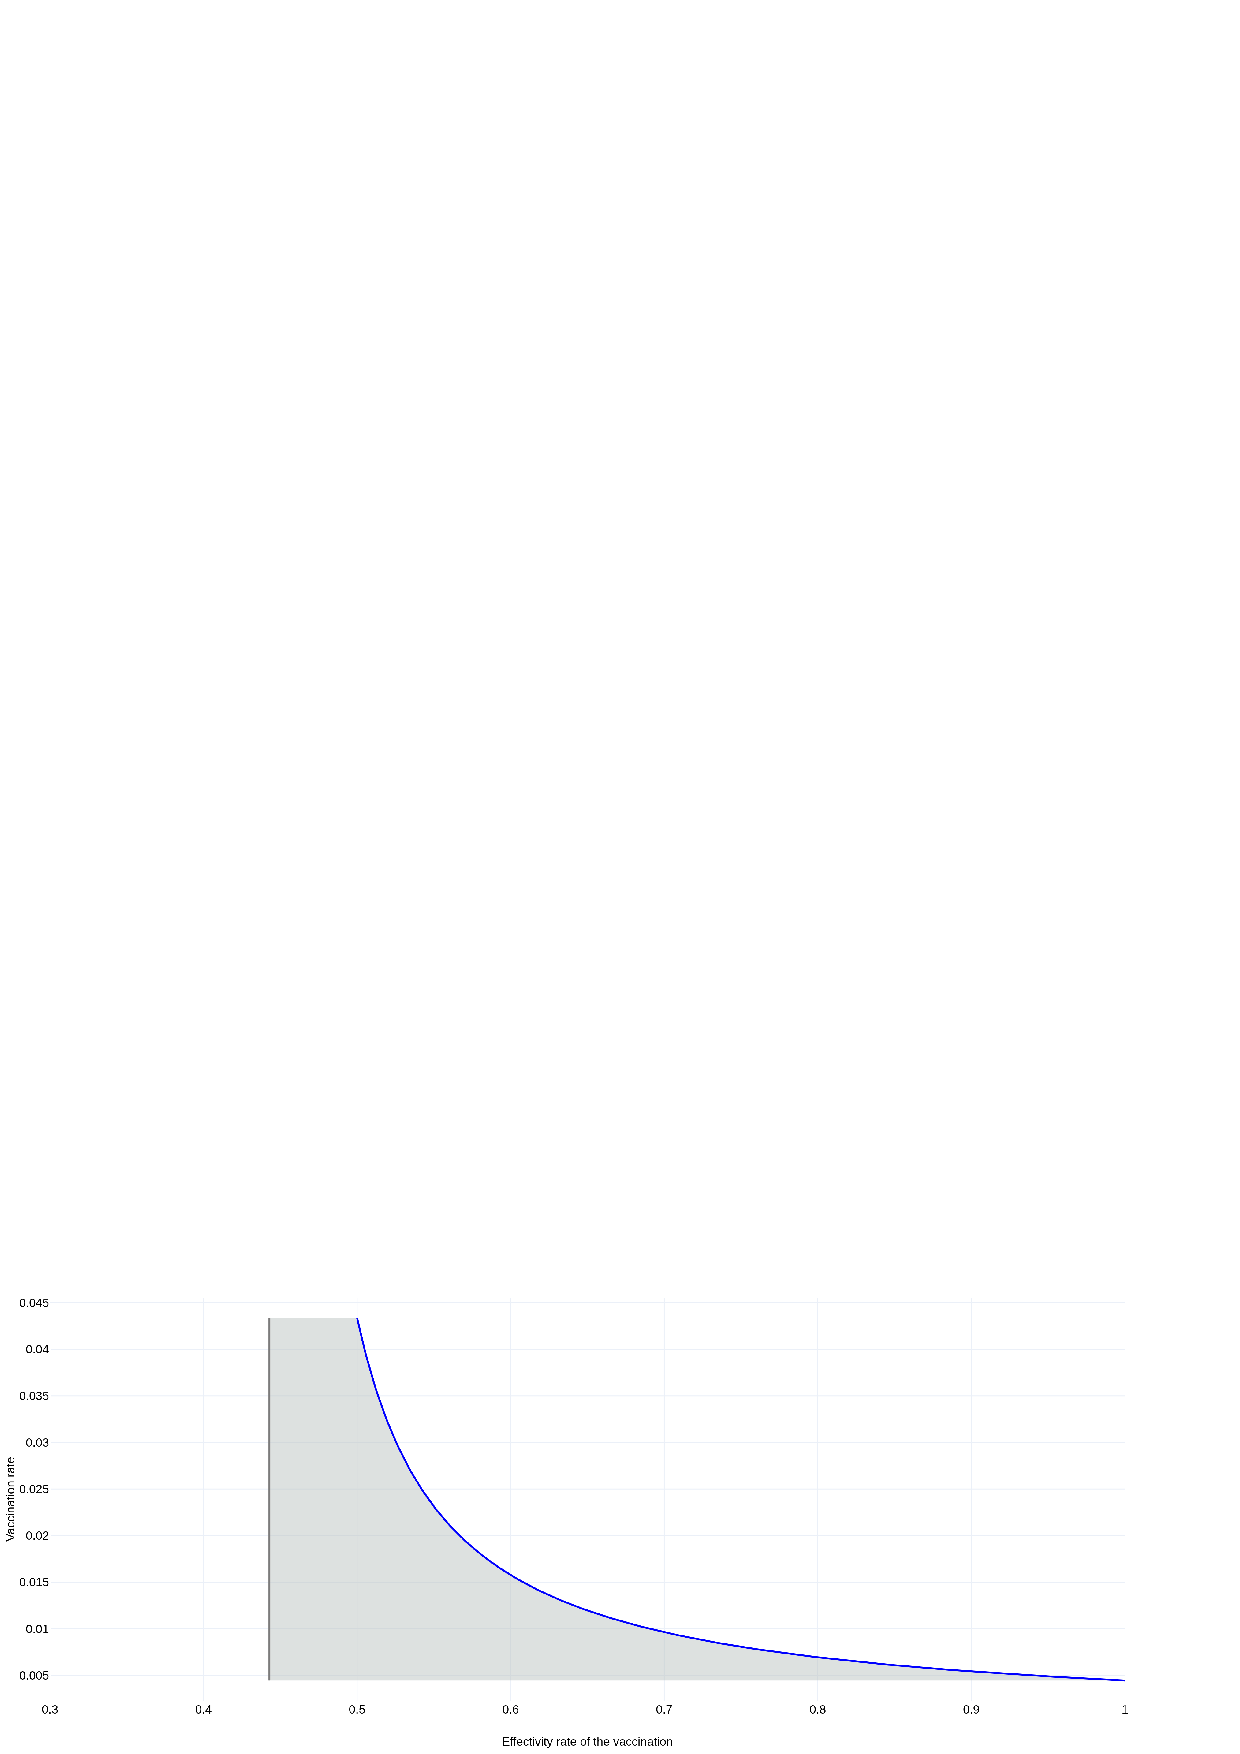
\includegraphics[scale=0.6]{R0-2D.png}
    \caption{
        Vaccine efficacy versus vaccination rate feasibility.
        In the shaded region $R_V>1 $ and in the white region $ R_V <1 $.
        Note that, for our scenario, with a $50$ percent vaccine effectiveness
        and an adequate vaccination rate, it is possible to reduce the $ R_V $
        value below one. The orange region is unfeasible.}
    \label{R0-2D}
\end{figure*}

\subsection{Baseline vaccination rate formulation}
Vaccination policies to reach a given coverage of a
certain percentage of the population in a given period is of great importance.
In this sense, we refer to this vaccination constant rate as the base vaccination
rate, denoted by $ \lambda_{Vbase}$.

Let $W(t)$ be the normalized unvaccinated population at time $t$, we consider
that at $t=0$ no person has been vaccinated, which implies $W(0)=1$.
Then, by assuming that we vaccinate individuals at a constant rate $\lambda_{Vbase}$
proportional to the actual population, we have that $W(t)$ satisfies the equation
$$
\dot{W}(t)=-\lambda_{Vbase} W(t)
\qquad \qquad \textrm{with} \qquad\qquad {W(0)=1}
$$
or $W(t)=e^{-\lambda_{Vbase}t}$. It implies that the number of vaccinated individuals
at time $t$ is given by $V(t)=1-e^{-\lambda_{Vbase}t}$. Then, if we look
to reach a coverage $x_{coverage}$ at a horizon time $T$, it follows that $\lambda_{Vbase}$
satisfies the equation
\begin{equation}
    \label{eqn:lambda_base}
    \begin{aligned}
        & x_{coverage} =
            1 - \exp(-\lambda_{Vbase} \ T)
        \\
        \textrm{thus }&
        \\
        & \lambda_{Vbase} =
            \dfrac{
                -\ln{(1 - x_{coverage})}
            }{T} .
    \end{aligned}
\end{equation}
Observe that in the calculation of $\lambda_{Vbase}$, it is considered all
the population to be vaccinated. Vaccination is not applied to infective symptomatic
individuals. Therefore, \Cref{eqn:lambda_base} represents an approximation
of the vaccination scheme at constant rate.

\Cref{R0_contour}, shows the contour curves for $ R_0 $ considering it as a function
of the efficacy of the vaccine $ (\epsilon) $ and of the vaccination rate $ (\delta_V) $,
considering an immunity period induced by the vaccine of half year . The blue line,
correspond to the values of $\lambda_{Vbase}$ and we can see that with
this vaccination rate, no matter how effective the vaccine is, it is not possible
to reduce the value of $R_V$ below one. Purple lines show a scenario in
which it is possible to reduce the $R_V$ value below one, considering a vaccine efficacy of
\num{0.8} and a  vaccination rate of \num{0.7}.
The figure shows plausible combinations of $\epsilon$ and $\lambda_V$ values
in order to reduce the value of $R_V$ below one.

Note that a vaccine efficacy of \SI{50}{\percent} or more is required so that, with an
adequate vaccination rate, the $R_V$ value can be reduced below one.

\begin{figure*}[tbh]
    \centering
    \includegraphics[scale=.50]{R0_contour.png}
    \caption{
        Contour plot  of $R_V$ like function of $ \epsilon $ and $ \lambda_V $ and with
        immunity average time by vaccination of half year. Dark green line represents the
        value of $\lambda_{Vbase}=\num{0.000611}$, corresponding to a coverage
        $x_{coverage} = \num{0.2}$ and a
        horizon time $T=\num{365}$. Red lines show a scenario in which it is possible to
        reduce the $R_V$ value below one, considering a vaccine efficacy of
        \num{0.8} and a vaccination rate
        of \num{0.7}.}
    \label{R0_contour}
\end{figure*}

In the next section, the optimal control theory will be applied to propose optimal
vaccination dynamics that minimize the number of cases of symptomatic infection and deaths
due to the disease.